\begin{frame}{Pipeline empleado}
	\begin{figure}[H]
		\centering
		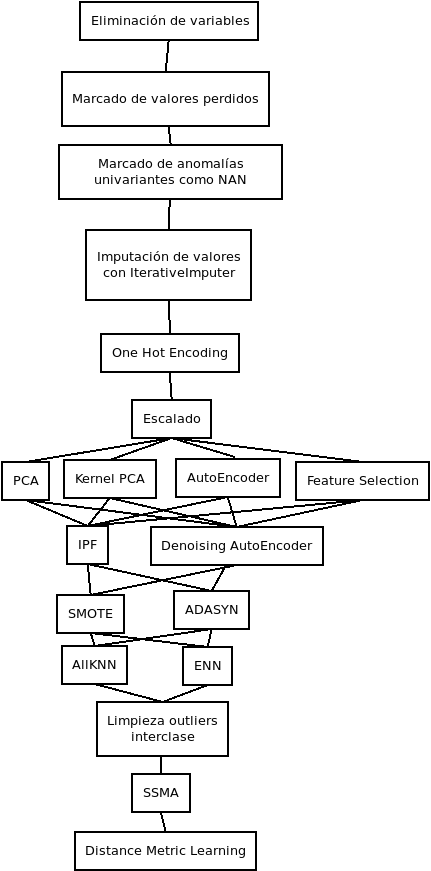
\includegraphics[scale=0.25]{./figures/knn/pipeline.png}
	\end{figure}
\end{frame}

\begin{frame}{Pipeline con mejor resultado}
	\begin{figure}[H]
		\centering
		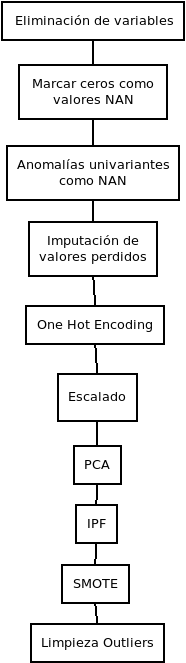
\includegraphics[scale=0.33]{./figures/knn/pipeline_final.png}
	\end{figure}
\end{frame}

\begin{frame}{Explicación de las técnicas}
	\vspace{10px}
	\pause
	\metroset{block=fill}
	\begin{block}{Eliminación de variables}
		Elimino las variables wpt\_name, subvillage, scheme\_name, funder, installer, ward, amount\_tsh y num\_private.
	\end{block}
	\pause
	\begin{block}{Marcado de anomalías como valores perdidos}
		En cada columna se calcula la media y la desviación típica. Aquellos datos que se salgan del intervalo $[media-5std, media+5std]$ se marcan como NAN.
	\end{block}
	\pause
	\begin{block}{Imputación iterativa}
		Empleamos una imputación iterativa sobre los valores perdidos.
	\end{block}
	\pause
	\begin{block}{PCA}
		Aplicamos PCA pero sólo sobre las columnas categóricas. El objetivo es explicar las variables categóricas mejor que en su codificación original. Reducimos a 44 variables todas las categóricas.
	\end{block}
\end{frame}

\begin{frame}{Explicación de las técnicas}
	\vspace{10px}
	\pause
	\metroset{block=fill}
	\begin{block}{IPF}
		Ejecutamos un IPF para limpiar el ruido con 4 iteraciones.
	\end{block}
	\pause
	\begin{block}{SMOTE}
		Hacemos un oversampling de las clases ''functional needs repair'' y ''non functional'' a 7500 y 22000 con respecto a 23500 de la clase ''functional'' con $k=7$.
	\end{block}
	\pause
	\begin{block}{Limpieza Outliers}
		Hacemos una limpieza de anomalías por cada clase eliminando el 1\% más anómalo según KNN con $k=7$ y la métrica de la mayor distancia.
	\end{block}
\end{frame}

\begin{frame}{Visualización de las técnicas}
	\begin{tabular}{ccc}
		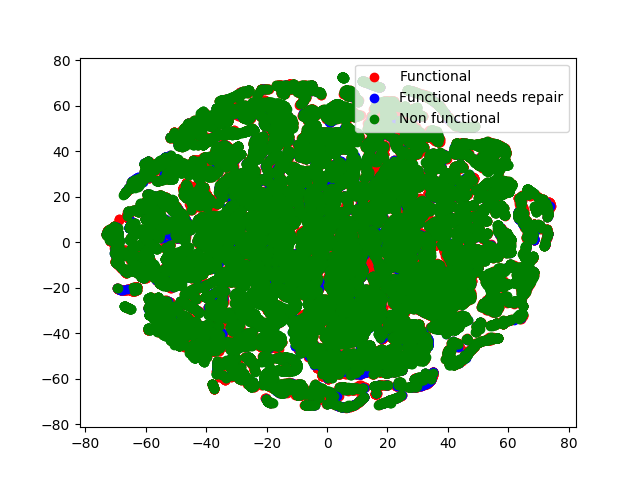
\includegraphics[scale=0.21]{./figures/knn/raw_2d.png} & 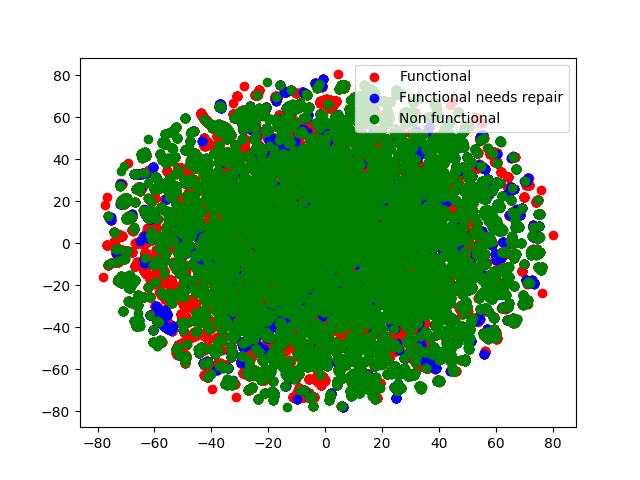
\includegraphics[scale=0.21]{./figures/knn/scaled_2d.png} & 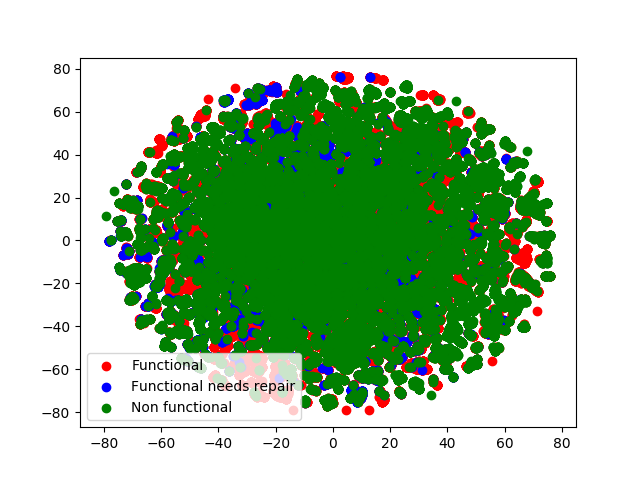
\includegraphics[scale=0.21]{./figures/knn/PCA_2d.png} \\
		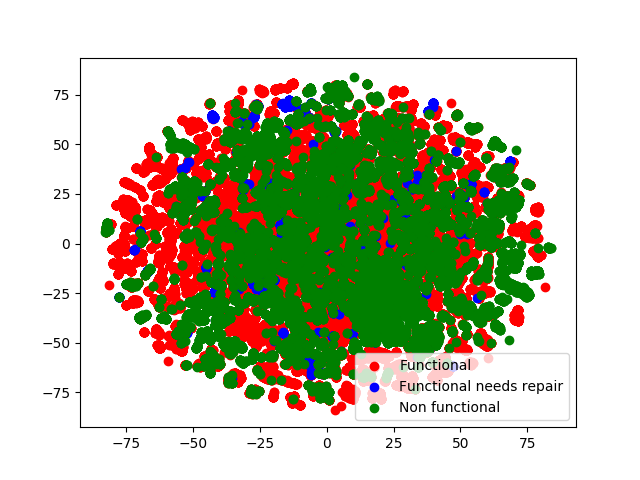
\includegraphics[scale=0.21]{./figures/knn/IPF_2d.png} & 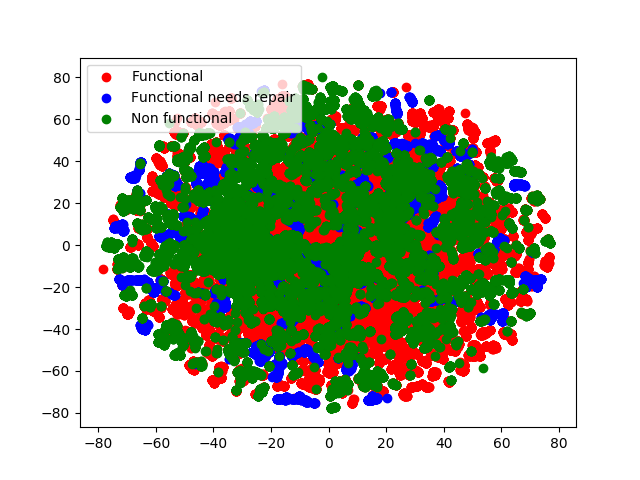
\includegraphics[scale=0.21]{./figures/knn/SMOTE_2d.png} & 
		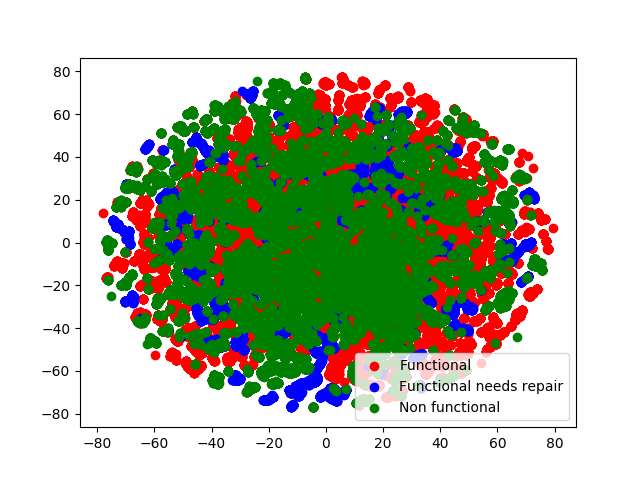
\includegraphics[scale=0.21]{./figures/knn/anomalias_knn_2d.png}
	\end{tabular}
\end{frame}

\begin{frame}{Elección del K y dimensionalidad de PCA}
	\vspace{10px}
	\pause
	\metroset{block=fill}
	\begin{block}{Parámetros del modelo}
		Se hace validación cruzada y se toma tanto el mejor valor de $k$ para KNN como el mejor valor de dimensionalidad para PCA.
		
		Estos parámetros son $k=1$ y $dim=44$.
	\end{block}
\end{frame}

\begin{frame}{Posición en DrivenData}

	\begin{figure}[H]
		\centering
		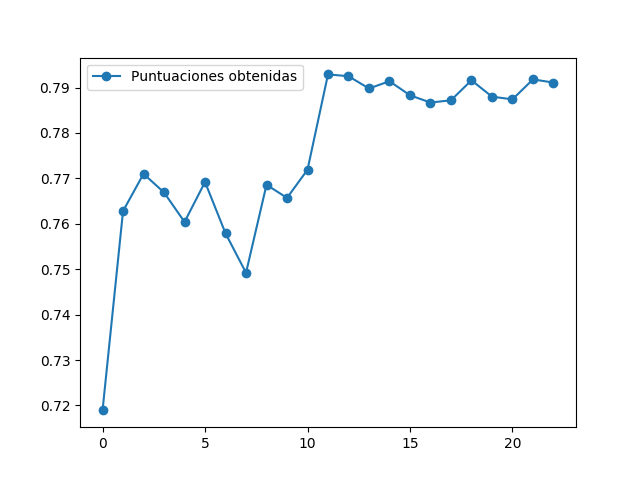
\includegraphics[scale=0.45]{./figures/knn/scores.png}
	\end{figure}

	\centering
	Puntuación final obtenida: 79.29\%
	
	Ranking final: 1729
	
	Número de subidas: 23
    
\end{frame}

